%%%%%%%%%%%%%%%%%%%%%%%%%%%%%%%%%%%%%%%%%
% Class Notes Template
% LaTeX Template
% By: Ryan Grove
%%%%%%%%%%%%%%%%%%%%%%%%%%%%%%%%%%%%%%%%%

%----------------------------------------------------------------------------------------
%	PACKAGES AND OTHER DOCUMENT CONFIGURATIONS
%----------------------------------------------------------------------------------------

\documentclass[paper=a4, fontsize=11pt]{scrartcl} % A4 paper and 11pt font size

\usepackage[T1]{fontenc} % Use 8-bit encoding that has 256 glyphs
\usepackage{fourier} % Use the Adobe Utopia font for the document - comment this line to return to the LaTeX default
\usepackage[english]{babel} % English language/hyphenation
\usepackage{amsmath,amsfonts,amsthm} % Math packages

\usepackage{lipsum} % Used for inserting dummy 'Lorem ipsum' text into the template

\usepackage{sectsty} % Allows customizing section commands
\allsectionsfont{\centering \normalfont\scshape} % Make all sections centered, the default font and small caps

\usepackage{fancyhdr} % Custom headers and footers
\pagestyle{fancyplain} % Makes all pages in the document conform to the custom headers and footers
\fancyhead{} % No page header - if you want one, create it in the same way as the footers below
\fancyfoot[L]{} % Empty left footer
\fancyfoot[C]{} % Empty center footer
%\fancyfoot[R]{\thepage} % Page numbering for right footer
\renewcommand{\headrulewidth}{0pt} % Remove header underlines
\renewcommand{\footrulewidth}{0pt} % Remove footer underlines
\setlength{\headheight}{13.6pt} % Customize the height of the header

\numberwithin{equation}{section} % Number equations within sections (i.e. 1.1, 1.2, 2.1, 2.2 instead of 1, 2, 3, 4)
\numberwithin{figure}{section} % Number figures within sections (i.e. 1.1, 1.2, 2.1, 2.2 instead of 1, 2, 3, 4)
\numberwithin{table}{section} % Number tables within sections (i.e. 1.1, 1.2, 2.1, 2.2 instead of 1, 2, 3, 4)

\setlength\parindent{0pt} % Removes all indentation from paragraphs - comment this line for an assignment with lots of text

\usepackage{lastpage}
\usepackage{fancyhdr}
\cfoot{\thepage\ of \pageref{LastPage}}

\def\v{\hbox{$\mathbf v$}}
\def\w{\hbox{$\mathbf w$}}
\def\u{\hbox{$\mathbf u$}}
\def\x{\hbox{$\textbf{x}$}}
\def\z{\hbox{$\mathbf z$}}
\def\a{\hbox{$\mathbf a$}}
\def\b{\hbox{$\mathbf b$}}
\def\L{\hbox{$\mathcal L$}}
\def\C{\hbox{$\mathbb C$}}
\def\B{\hbox{$\mathcal B$}}
\def\R{\hbox{$\mathbb R$}}
\def\X{\hbox{$\underline X$}}
\def\Q{\hbox{$\mathbb Q$}}
\def\R{\hbox{$\mathbb R$}}
\def\N{\hbox{$\mathbb N$}}
\def\C{\hbox{$\mathbb C$}}
\def\0{\hbox{$\mathbf 0$}}
\def\Y{\hbox{$\underline Y$}}
\def\a{\hbox{$\mathbf a$}}
\def\u{\hbox{$\mathbf u$}}
\def\w{\hbox{$\mathbf w$}}
\def\y{\hbox{$\mathbf y$}}
\def\X{\hbox{$\underline X$}}
\def\dd{\hbox{$\partial $}}
\def\B{\hbox{$\mathcal B$}}
\def\F{\hbox{$\mathcal F$}}
\def\L{\hbox{$\mathcal L$}}
\def\M{\hbox{$\mathcal M$}}
\def\D{\hbox{$\mathscr {D}$}}
\def\RR{\hbox{$\mathscr{R}$}}
\def\I{\hbox{$\mathcal I$}}

\usepackage{amssymb}
%\theoremstyle{plain}
\usepackage[margin = .75in]{geometry}
\newtheorem{claim}{Claim}
\newtheorem{theorem}{Theorem}[section]
\newtheorem{lemma}[theorem]{Lemma}
\newtheorem{proposition}[theorem]{Proposition}
\newtheorem{corollary}[theorem]{Corollary}
\newtheorem{problem}[theorem]{Problem}
%\theoremstyle{definition}
\newtheorem{definition}[theorem]{Definition}
%\theoremstyle{remark}
\newtheorem{remark}[theorem]{Remark}
\newtheorem{remarks}[theorem]{Remarks}
\newtheorem{example}[theorem]{Example}
\newcommand{\ds}{\displaystyle}
\newcommand{\ZZ}{\mathbb{Z}}
\newcommand{\QQ}{\mathbb{Q}}
\newcommand{\e}{\varepsilon}
\newcommand{\bbf}{\textbf}
\newcommand{\p}{\parallel}
\usepackage{color}
\newcommand{\field}[1]{\mathbb{#1}}
\usepackage{amsmath}
\usepackage{amsthm}
\usepackage{amssymb}
\usepackage{mathrsfs}
\usepackage{cancel}
\usepackage{upgreek}
\usepackage{graphicx}
\usepackage{multirow}
\usepackage{setspace}
\usepackage{url}
\usepackage{subfigure}
\usepackage{enumerate}
\usepackage{cases}
\usepackage{mathrsfs}
\usepackage{rotating}

%----------------------------------------------------------------------------------------
%	TITLE SECTION
%----------------------------------------------------------------------------------------

\newcommand{\horrule}[1]{\rule{\linewidth}{#1}} % Create horizontal rule command with 1 argument of height

\title{	
\normalfont \normalsize 
\textsc{Ryan Grove, Clemson University, MATH1080 - 9} \\ [25pt] % Your name, university, class
\horrule{0.5pt} \\[0.4cm] % Thin top horizontal rule
\huge Section 10.4: Area \& Lengths in Polar Coordinates \\ % The assignment title
\horrule{2pt} \\[0.5cm] % Thick bottom horizontal rule
}

\author{Date:} % The due date

\date{\normalsize April 19, 2016} % A custom date

\begin{document}

\maketitle % Print the title

\begin{flushleft}
\begin{tabular}{l l}
Name: \rule{3.2in}{.01cm}  & {}%Table number: \rule{1in}{.01cm}\\
\end{tabular}
\end{flushleft}

%----------------------------------------------------------------------------------------
%	Lecture
%----------------------------------------------------------------------------------------

\section*{\textbf{Lecture:}}

\[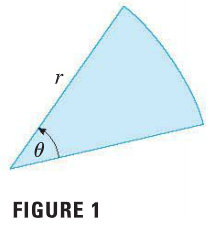
\includegraphics[scale=0.45]{10-4pic1.png} \quad \quad 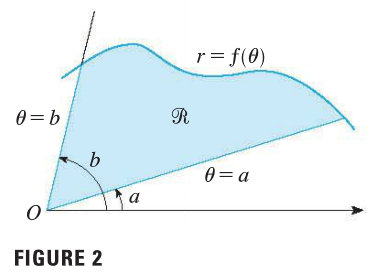
\includegraphics[scale=0.45]{10-4pic2.png} \quad \quad 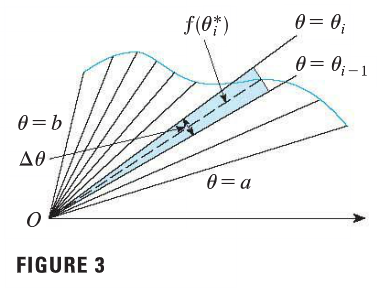
\includegraphics[scale=0.45]{10-4pic3.png}\]


In this section we develop the formula for the area of a region whose boundary is given by a polar equation. We need to use the formula for the \underline{area of a sector of a circle}:

\[A = \underline{\hspace{1in}}\]

where, as in Figure 1, $r$ is the radius and $\theta$ is the radian measure of the central angle.\\
\indent

Let $\mathcal{R}$ be the region, illustrated in Figure 2, bounded by the polar curve $r=f(\theta)$ and by the rays $\theta = a$ and $\theta = b$, where $f$ is a positive continuous function and where $0<b-a\leq 2\pi$. We divide the interval $[a,b]$ into $n$ equal width subintervals with endpoints, $\theta_0,\theta_1,\theta_2,\ldots,\theta_n$ and width $\Delta \theta$. The rays $\theta_i$ then divide $\mathcal{R}$ into $n$ smaller regions with central angle $\Delta\theta = \theta_i - \theta_{i-1}$. If we choose $\theta_i^*$ in the $i$th subinterval $[\theta_{i-1},\theta_i]$, then the area $\Delta A_i$ of the $i$th region is approximated by the area of the sector of a circle with central angle $\Delta \theta$ and radius $f(\theta_i^*)$.\\
\indent

Thus from the Formula above we have,

\[\Delta A_i \approx \ds\frac{1}{2}[f(\theta_i^*)]^2\Delta\theta\]

and so an approximation to the total area $A$ or $\mathcal{R}$ is

\[A\approx \ds\sum_{i=1}^n \ds\frac{1}{2}[f(\theta_i^*)]^2\Delta\theta.\]

It appears from Figure 3 that the approximation improves as $n\to\infty$, and as we've seen before, the sums are Riemann sums for the function $g(\theta)=\ds\frac{1}{2}[f(\theta)]^2$, so

\[\ds\lim_{n\to\infty}\ds\sum_{i=1}^n\ds\frac{1}{2}[f(\theta_i^*)]^2\Delta\theta = \underline{\hspace{1.25in}}.\]
\indent

Therefore, we have that the area $A$ of the polar region $\mathcal{R}$ is

\[\boxed{ \quad A = \ds\int_a^b \ds\frac{1}{2}[f(\theta)]^2 d\theta  = \ds\int_a^b \ds\frac{1}{2}r^2 d\theta \quad }\]
\indent

\newpage
\underline{Example 1}: Find the area enclosed by one loop of the four-leaved rose $r=\cos2\theta$.\\
\indent

$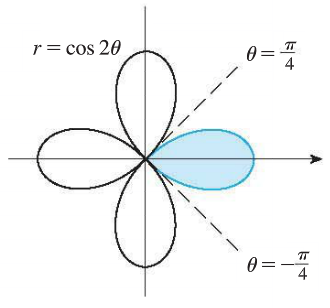
\includegraphics[scale=0.4]{10-4pic4.png}$
\indent

\vspace{1.5in}

\underline{Example 2}: Find the area of the region that lies inside the circle $r=3\sin\theta$ and outside the cardioid $r=1+\sin\theta$.\\
\indent

$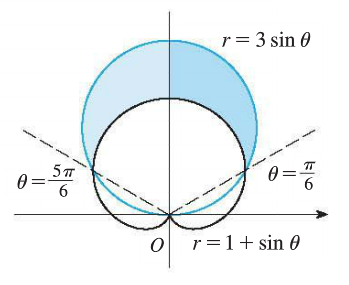
\includegraphics[scale=0.4]{10-4pic5.png}$

\newpage

Example 2 illustrated the procedure for finding the area of the region bounded by two polar curves. In general, let $\mathcal{R}$ be a region, as illustrated in Figure 6, that is bounded by curves with polar equations $r=f(\theta), r=g(\theta), \theta=a,$ and $\theta=b$, where $f(\theta)\geq g(\theta)\geq 0$ and $0<b-a\leq 2\pi$. The area $A$ of $\mathcal{R}$ is found by subtracting the area inside $r=g(\theta$ from the area inside $r=f(\theta$, so we have:
\vspace{-10pt}
\begin{align*}
A &= \ds\int_a^b \ds\frac{1}{2}[f(\theta)]^2 d\theta - \ds\int_a^b \ds\frac{1}{2}[g(\theta)]^2 d\theta\\
&= \ds\frac{1}{2}\ds\int_a^b([f(\theta)]^2 - [g(\theta)]^2)d\theta
\end{align*}
\vspace{-30pt}

\[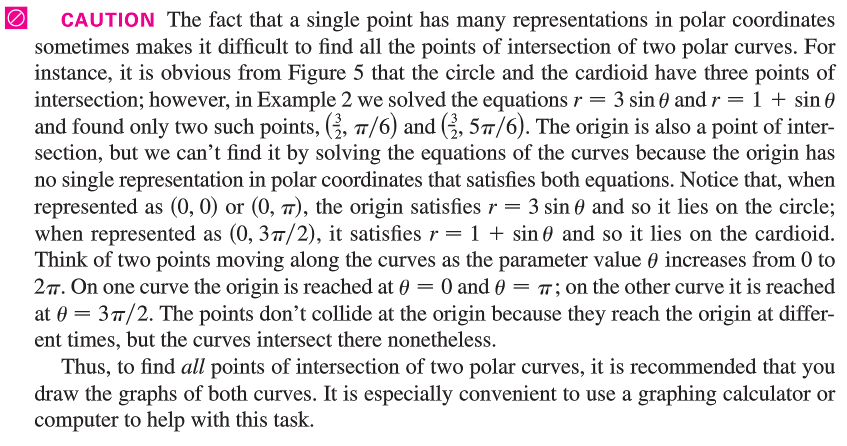
\includegraphics[scale=0.45]{caution.png}\]

\underline{Example 3}: Find all points of intersection of the curves $r=\cos 2\theta$ and $r=\ds\frac{1}{2}$.\\
\indent

\textbf{Solving the Equations}:\\

\vspace{1.5in}

\textbf{Graphically}: \\
\indent

\quad $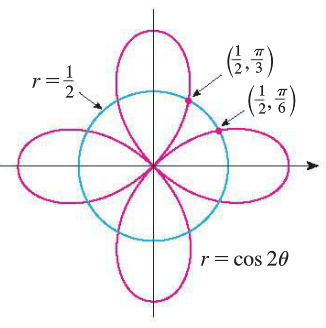
\includegraphics[scale=0.45]{10-4pic7.png}$

\vspace{-140pt}

\hspace{2.5in} We can see here that the curves have four other points of \\
\hspace{2.5in} intersection--namely,
\[\hspace{2in} (\ds\frac{1}{2},\ds\frac{\pi}{3}),(\ds\frac{1}{2},\ds\frac{2\pi}{3}),(\ds\frac{1}{2},\ds\frac{4\pi}{3}), \text{ and } (\ds\frac{1}{2},\ds\frac{5\pi}{3}).\]
\hspace{2.5in} These can be found using symmetry or by noticing that \\
\hspace{2.5in}another equation of the circle is $r=-\ds\frac{1}{2}$ and then solving the  \\
\hspace{2.5in} equations $r=\cos 2\theta$ and $r=-\ds\frac{1}{2}$.



%----------------------------------------------------------------------------------------

\end{document}